% Options for packages loaded elsewhere
\PassOptionsToPackage{unicode}{hyperref}
\PassOptionsToPackage{hyphens}{url}
%
\documentclass[
]{article}
\title{Report}
\author{Maja}
\date{2023-03-26}

\usepackage{amsmath,amssymb}
\usepackage{lmodern}
\usepackage{iftex}
\ifPDFTeX
  \usepackage[T1]{fontenc}
  \usepackage[utf8]{inputenc}
  \usepackage{textcomp} % provide euro and other symbols
\else % if luatex or xetex
  \usepackage{unicode-math}
  \defaultfontfeatures{Scale=MatchLowercase}
  \defaultfontfeatures[\rmfamily]{Ligatures=TeX,Scale=1}
\fi
% Use upquote if available, for straight quotes in verbatim environments
\IfFileExists{upquote.sty}{\usepackage{upquote}}{}
\IfFileExists{microtype.sty}{% use microtype if available
  \usepackage[]{microtype}
  \UseMicrotypeSet[protrusion]{basicmath} % disable protrusion for tt fonts
}{}
\makeatletter
\@ifundefined{KOMAClassName}{% if non-KOMA class
  \IfFileExists{parskip.sty}{%
    \usepackage{parskip}
  }{% else
    \setlength{\parindent}{0pt}
    \setlength{\parskip}{6pt plus 2pt minus 1pt}}
}{% if KOMA class
  \KOMAoptions{parskip=half}}
\makeatother
\usepackage{xcolor}
\IfFileExists{xurl.sty}{\usepackage{xurl}}{} % add URL line breaks if available
\IfFileExists{bookmark.sty}{\usepackage{bookmark}}{\usepackage{hyperref}}
\hypersetup{
  pdftitle={Report},
  pdfauthor={Maja},
  hidelinks,
  pdfcreator={LaTeX via pandoc}}
\urlstyle{same} % disable monospaced font for URLs
\usepackage[margin=1in]{geometry}
\usepackage{graphicx}
\makeatletter
\def\maxwidth{\ifdim\Gin@nat@width>\linewidth\linewidth\else\Gin@nat@width\fi}
\def\maxheight{\ifdim\Gin@nat@height>\textheight\textheight\else\Gin@nat@height\fi}
\makeatother
% Scale images if necessary, so that they will not overflow the page
% margins by default, and it is still possible to overwrite the defaults
% using explicit options in \includegraphics[width, height, ...]{}
\setkeys{Gin}{width=\maxwidth,height=\maxheight,keepaspectratio}
% Set default figure placement to htbp
\makeatletter
\def\fps@figure{htbp}
\makeatother
\setlength{\emergencystretch}{3em} % prevent overfull lines
\providecommand{\tightlist}{%
  \setlength{\itemsep}{0pt}\setlength{\parskip}{0pt}}
\setcounter{secnumdepth}{-\maxdimen} % remove section numbering
\ifLuaTeX
  \usepackage{selnolig}  % disable illegal ligatures
\fi

\begin{document}
\maketitle

\#Introduction

\emph{Trauma}

Trauma, clinically defined as physical injury and the body´s associated
response, is the most common cause of death in the first four decades of
life. It kills around 4.4 million people around the globe {[}@who2021{]}
and in Sweden, almost 10,000 people suffer from severe trauma
yearly.{[}@swetrau2021{]} Trauma is generally divided into two
categories based on the mechanism of injury; penetrating (stab wounds or
gunshots) and blunt ( e.g.~car accidents, falls and interpersonal
violence) {[}@Santos2018{]}. Overall, brain injury is the most common
cause of trauma related death, counting for 58,6 percent. In 2021, 62
percent of patients passing from blunt violence in Sweden did so due to
damage of the brain. For penetrating trauma, the equivalent figure was
22 percent. {[}@ghorbani2014{]}. In addition, brain injuries are largely
associated with non-preventable mortality {[}@roy2017{]} and are hence
weighing on mortality statistics of both cohort.Thereof, brain injuries
are sometimes better separated and evaluated as a category of its own.

\emph{AIS score}

The abbreviated injury scale (AIS) is a 6-point scale scoring system
ranking the severity of injury for five anatomic regions, and has been
implemented as standard categorization of injury for trauma patients
internationally {[}@gennarelli2006, @AIS2023{]}. The American College of
Surgeons (ASC) Trauma quality improvement program (TQIP) has further
used the AIS-system to create definitions for patient cohorts (blunt,
penetrating, brain injury){[}@Blackmore2019,{]}. This facilitates
comparability and thereby studies of trauma patient data
internationally.

\emph{Trauma system}

A trauma system is a coordinated network of healthcare providers and
resources designed to provide timely and effective care to patients with
traumatic injuries. Trauma systems have a long tradition within the
military but were not implemented in civil health care until the
1960s-1970s when the report ``Accidental Death and Disability: The
Neglected Disease of Modern Society'' was published in the US
{[}@choi2021{]}. Since then, trauma systems have been put into practice
in most modern countries, improving mortality and morbidity for severely
injured patients {[}@TraumaSystem2014{]}. The ACS provides guidelines
for how the system should be structured. In general, the system consists
of four components; (i) pre-hospital care, (ii) hospital care at a
trauma center, (iii) post-hospital care and (iv) injury
prevention.{[}@TraumaSystem2014{]}.

\emph{Trauma centers}

Trauma centers are essential to the trauma system and constitute medical
facilities that meet specific criteria established by the ACS. There are
five levels of trauma centers, where each level refers to the kinds of
resources available at the center and number of patients admitted
yearly. Level 1 trauma centers provide the highest level of care and are
equipped for every aspect of injury around the clock {[}@ATS2023{]}.
Apart from medical resources such as operating rooms, standby trauma
teams, advanced x-rays and well-stocked blood banks, level-1 trauma
centers should engage in quality assessments and improvement programs
for trauma care {[}@Darnell2022{]}.

\emph{M\&M conferences}

Mortality and Morbidity (M\&M) conferences are recurring meetings at
trauma centers. At conference, a multidisciplinary team of qualified
doctors and nurses evaluate selected patient cases to evaluate whether
death could have been prevented in cases with fatal outcome. The team
also discusses other potential errors in the care of the patient with
the aim to identify Opportunities for improvement and cautionary actions
to be taken for better care throughout the entire process, from onset of
injury to rehab {[}@Sanddal2011{]}. Whether a M\&M conference has been
held within 30 days after a trauma occasion, is often used as a quality
measure of care. M\&M-conferences should be an integrated part of trauma
operations at all level-1 trauma centers {[}@Swetrau2020{]}.

\emph{Opportunities for improvement}

Opportunities for improvement (OFI) is an established concept within
trauma care evaluation and can be defined as all deficiencies or
aberrations from guidelines at any stage of care in a trauma system that
could be avoided through optimized action {[}@bixby2016{]}. OFIs can
thus be identified in all care processes regardless of whether patient
outcome is in line with what could have been expected or not. In events
where trauma leads to death, mortality can be sorted into either
preventable or non-preventable, where preventable mortality is defined
as loss of life that likely would have been avoided if one or more
errors in the trauma system would have been corrected {[}@heim2016{]}.

\emph{Current landscape}

To date a variety of studies based on OFIs have been conducted with the
aim to identify recurrent errors for specific patient cohorts or trauma
facilities. Socioeconomic, cultural and geographic issues, trauma
characteristics and healthcare vary between countries and rural/city
areas {[}@jiang2020, @jeppesen2020{]}. In Sweden surgical care is highly
centralized and no uniform national organization for trauma care is at
place. This makes evaluation of competence and performance at site
crucial to maintain high quality and avoid unnecessary risks for the
patient {[}@strommer2022{]}. Sweden further stand out from other western
countries with cold climate, fewer cases of serious trauma annually and
long distances to trauma centers, as few hospitals are equipped to treat
trauma-1 patients {[}@jeppesen2020, @steinvik2022{]}.

As mentioned earlier, the ACS have sorted trauma injuries into patient
cohorts according to the AIS system. To date, Swedish registry studies
on OFIs have mainly looked at three cohorts: blunt multisystem/single
trauma, penetrating trauma and traumatic brain injury {[}@ghorbani2014,
@strommer2022{]}. Since the most common cause of death among patients
suffering from blunt trauma is injury to the brain, an overlap between
cohorts occur when studying patients suffering multisystem trauma
without distinction between the brain and other areas of injury. In this
study, the blunt multisystem cohort is therefore analyzed both with and
without traumatic brain injury to avoid bias and to establish a clearer
understanding for preventability of death.

In addition, previous studies of the trauma registry have used OFI as a
composite measure for all potential lapses leading to un-optimal care.
Although this approach offers insight to whether opportunities for
improvement exist, it is insufficient in providing health care workers
with guidance to concrete actions that may improve care of trauma
patients. Hence, we have reviewed the correlation between specific OFIs
and patients cohorts.

\textbf{Aim}

This study hence aims at identifying specific OFIs for non-overlapping
cohorts (blunt multisystem trauma with brain injury, blunt multisystem
trauma without brain injury, penetrating trauma, isolated traumatic
brain injury) for more robust guidance in what specific actions could be
taken to improve trauma care for different patient cohorts.

\#Material and Methods

\textbf{Study design}

We conducted a registry-based cohort study on a merged dataset linking
data from the Swedish trauma registry SweTrau the trauma care quality
database at the Karolinska University Hospital. The combined data were
further assessed a through multinominal multivariable logistic
regression model to assess how clinical cohorts associate with OFIs.

\textbf{Setting}

From 2010, The Swedish Trauma society holds a national registry over
patients suffering serious trauma in Sweden. Patients included in the
registry have suffered traumatic events that have either triggered a
trauma alarm or generated injuries with a new injury severity score
(NISS) above 14.

In Sweden, the Karolinska University hospital covers the regions of
Stockholm, Gotland, Södermanland and Västmanland, equivalent to 3
million residents, which is just on pair with the minimum number of
patients needed to be recognized as a quality trauma centre
internationally. The hospital is also the only facility in Sweden to
qualify as a trauma-1 hospital by American standards
{[}@Fernelius2022{]}.

To detect non-optimal treatment, the Karolinska University hospital
evaluate trauma patients at a M\&M conference held by a
multidisciplinary board appointed by the hospital. The board consists of
a surgeon, an anaesthetist, a trauma nurse and in presence of specific
injuries (e.g., intracranial, orthopaedical or thoracic/vascular),
specialists from appropriate specialties. Competences involved in the
direct care of the patient are free to attend the conference but should
not take part in the review {[}@Swetrau2020{]}.

Patients are selected for conference in a multistage process with
escalating levels of reviews. All cases of mortality are passed directly
to conference, where the cause of death and whether it was preventable
or possibly preventable is decided. The review is then followed by
identification of OFIs, which serve as a foundation for enhancement of
care. The review process for non-mortality poor-outcomes has been
subsequently improved and formalised. In the years 2014-2017, trauma
patients were somewhat randomly selected and individually reviewed by a
specialised trauma nurse who made the call weather patients should be
escalated to conference. In 2017, the procedure was therefore formalized
with the introduction of audit filters.

\begin{figure}

{\centering 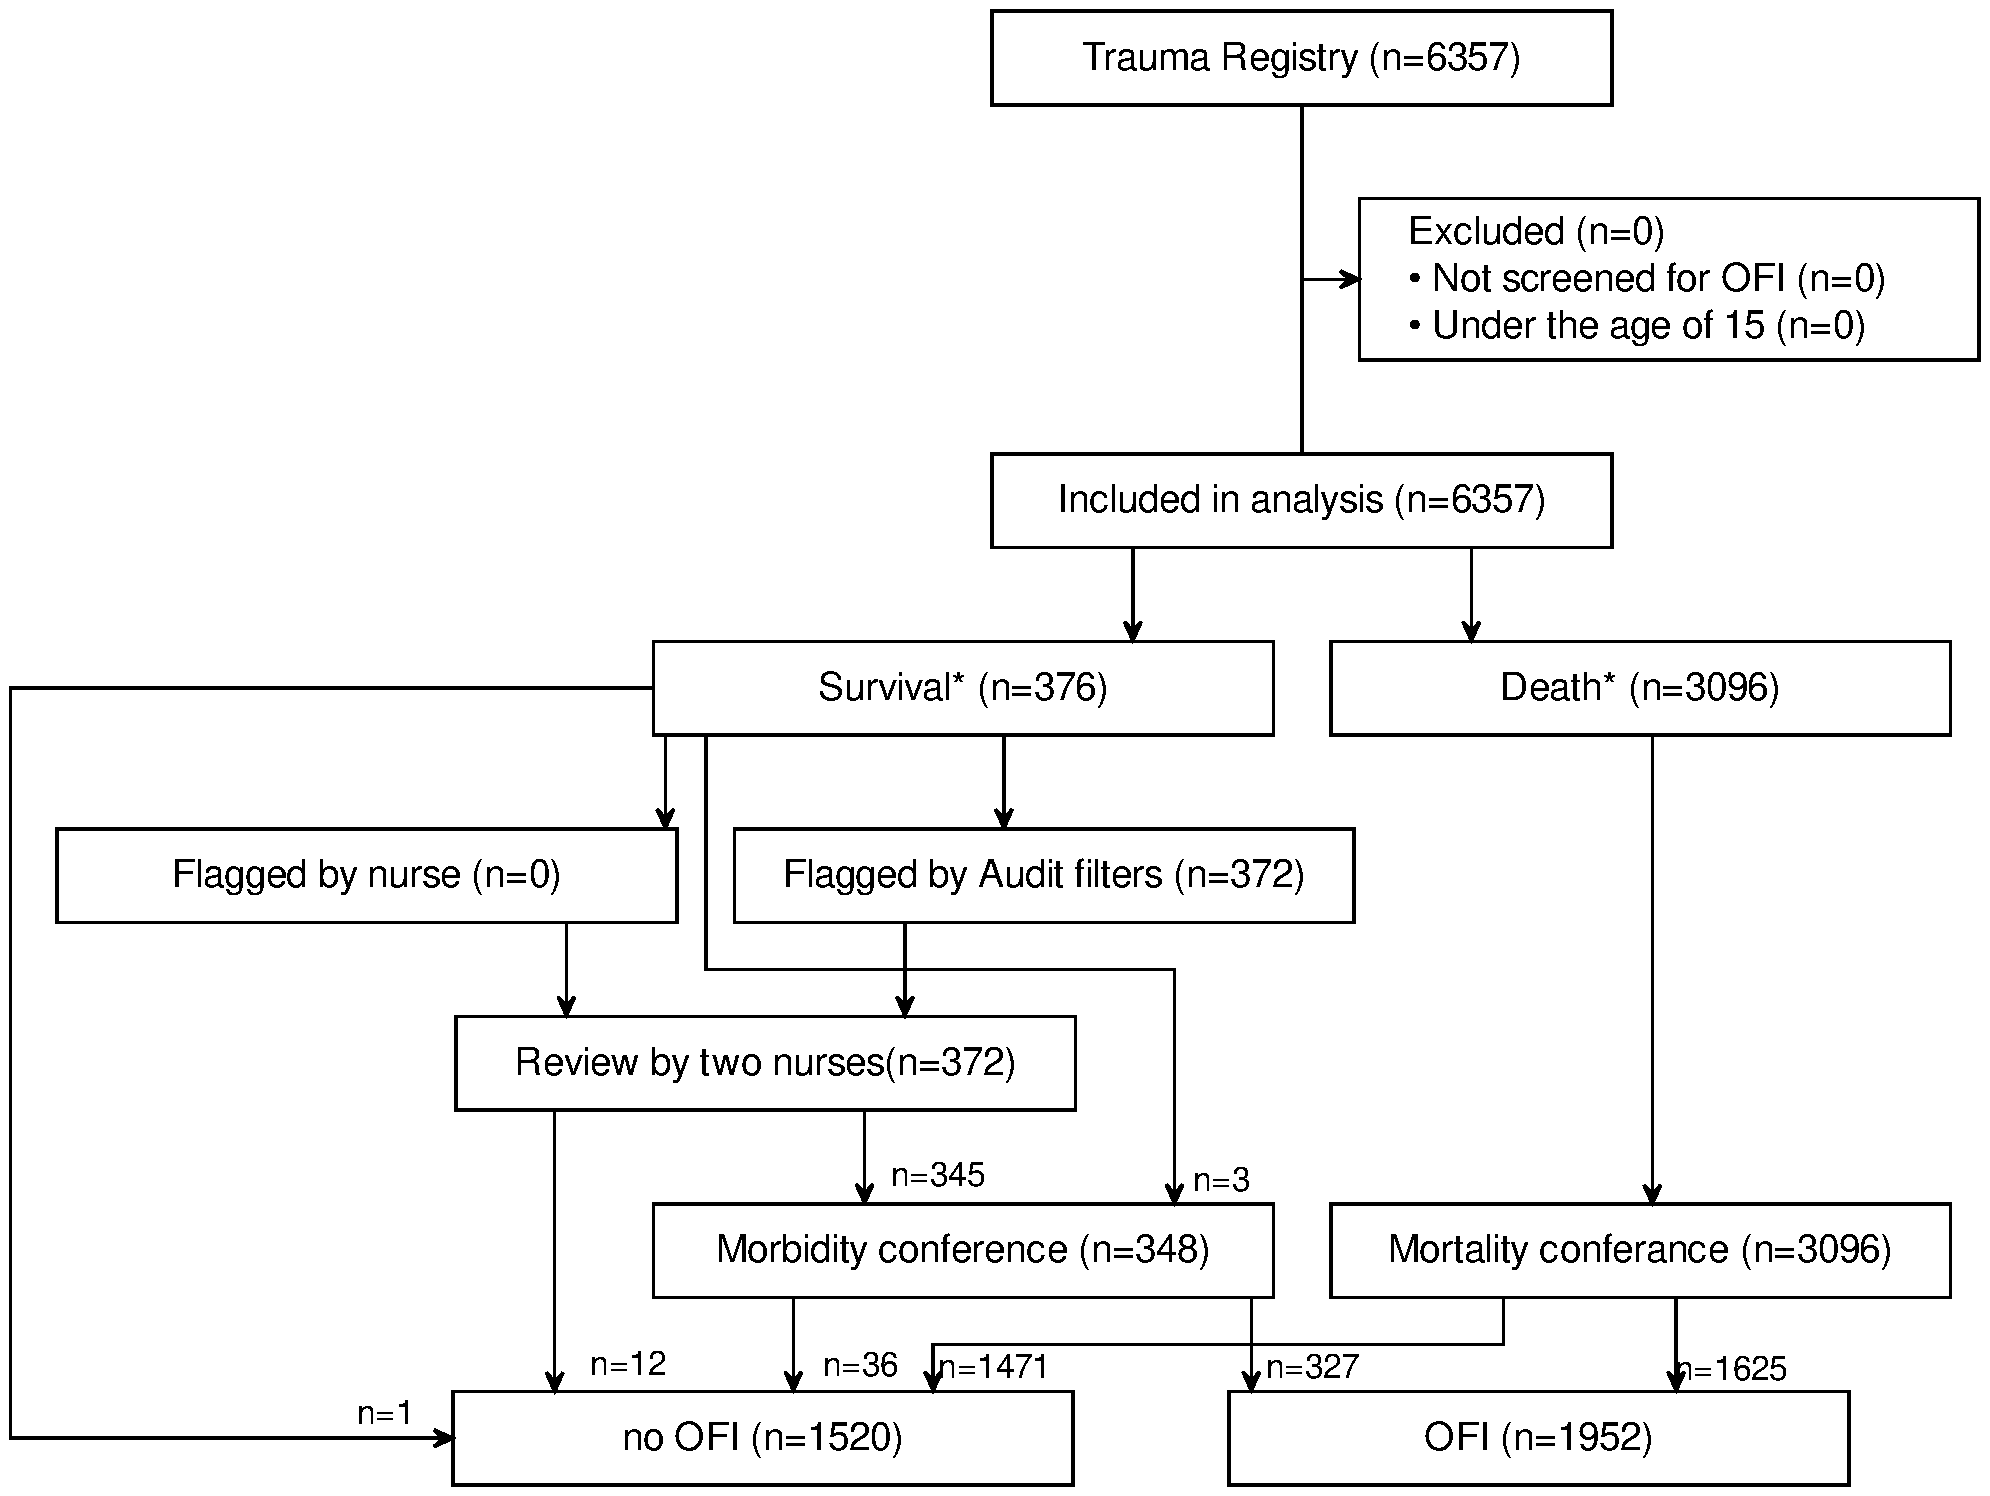
\includegraphics[width=1\linewidth]{ofi-flowchart} 

}

\caption{ Flowchart describing the exclusions made and the process of trauma cases from arrival until OFI decision.}\label{fig:ofi-flowchart}
\end{figure}

Audit filters, listed below, are specified conditions that all trauma
patients are automatically evaluated by. All patients captured by one or
more audit filters are then assessed by a nurse who identifies possible
glitches in care. Patients selected by the first nurse are then reviewed
again in a second round by two specialised nurses. If any OFIs are
identified in the second round, the patient is brought to a M\&M
conference for a final assessment of OFIs {[}@Swetrau2020{]}. Results
from the conference are stored in the Karolinska University hospital's
local quality care database.

Audit filters: * Systolic blood pressure \textless{} 90 * Glasgow coma
scale \textless{} 9 and not intubated. * Injury severity score
\textgreater{} 15 but not admitted to the intensive care unit * Time to
acute intervention \textgreater{} 60 minutes from arrival to hospital *
Time to computed tomography \textgreater{} 30 minutes from arrival to
hospital * No anticoagulant therapy within 72 hours after traumatic
brain injury * The presence of cardio-pulmonary resuscitation with
thoracotomy * The presence of a liver or spleen injury * Massive
transfusion, defined as 10 or more units of packed red blood cells
within 24 hours.

Study population We studied data of patients registered in both the
Swedish trauma registry from SweTrau and the trauma quality data base at
the Karolinska University hospital meeting the following criteria: *
Older than 15 years * A NISS \textgreater{} over 15 or an ISS
\textgreater9 * Being reviewed at an M\&M conference * Belonging to one
of the following cohorts: 1. blunt multisystem trauma with traumatic
brain injury 2. blunt multisystem trauma without traumatic brain injury
3. penetrating trauma 4. isolated severe traumatic brain injury

\emph{Variables}

The primary outcome was opportunities for improvements (OFI) detected by
the M\&M teams at the Karolinska University hospital. The variable is
categorical with the OFIs listed below as possible outcomes. The
exposure were different patient cohorts grouped by mechanism of injury,
(1) blunt multisystem trauma with traumatic brain injury, (2) blunt
multisystem trauma without traumatic brain injury, (3) penetrating
trauma, (4) isolated severe traumatic brain injury. Each cohort studied
was distinguished according to definitions provided by the ACS. 1. Blunt
multisystem trauma: Blunt trauma with injuries of Abbreviated Injury
Score (AIS) ≥ 3 in at least two of the following AIS body regions: head,
face, neck, thorax, abdomen, spine, or upper and lower extremities. 2.
Blunt multisystem trauma without traumatic brain injury: Blunt trauma
with injuries of Abbreviated Injury Score (AIS) ≥ 3 in at least two of
the following AIS body regions: face, neck, thorax, abdomen, spine, or
upper and lower extremities, but not head. 3. Penetrating trauma: At
least one AIS ≥ 3 injury in any of the following AIS body regions: neck,
thorax, and abdomen. 4. Isolated severe traumatic brain injury: Best GCS
within the first 24 h ≤ 8 OR Best motor score ≤ 3 within the first 24 h,
and one of: a. Abnormal CT brain (hematoma, contusion, swelling,
herniation, compression of basal cisterns b. Normal CT brain AND (Age
\textgreater{} 40 y OR SBP \textless90 mmHg on ED arrival) OR posturing
(GCS motor = 2, 3)

OFIs Identified at M\&M conference: * Missed injury/ problem at triage *
Problem with communication * Inadequate competence at site / No
neurosurgeon at site * problem with resources * Problem with management
(trauma criteria, logistics, problem with logistics and teqnique) *
Problem with Tertriry survey after stabilisation/resuscitation\\
* Wrong level of care * Exemplary treatment The model was adjusted for
gender, age and mortality. All variables with exception for age were
categorical.

Data sources/measurement The Swedish trauma registry SweTrau includes
all trauma patients with a NISS \textgreater15 or who have triggered an
alarm with trauma team activation in Sweden from 2010 to date. The
trauma care quality database at the Karolinska University hospital
includes data from trauma patients treated at the hospital from
2014-2021. In the years 2014-2017, patients all random set of patients
with an Injury severity score (ISS) of 9 or higher were included. From
2017, all patients included in the dataset have been reviewed at a M\&M
conference held at the the Karolinska University hospital.

In this study, all patients within the Karolinska University hospital
trauma quality registry reviewed at a M\&M conference were included. For
these patients, data from the Swedish trauma registry by SweTrau were
collected to a merged dataset. The merged dataset was then divided into
four cohorts; (1) blunt multisystem trauma with traumatic brain injury,
(2) blunt multisystem trauma without traumatic brain injury, (3)
penetrating trauma, (4) isolated severe traumatic brain injury.

\textbf{Bias}

To prevent bias, the multivariable regression model was developed using
a simulated scrambled dataset with random data. The algorithm for the
model was developed step-by-step and then evaluated by a trained
programmer and statistician before being applied on the real data.
Variables such as ID-number and name were scrambled and anonymised
throughout analysis of the real dataset.

\emph{Ethical considerations}

\emph{Study size}

\textbf{Results}

Of {[}\ldots{]} patients in the Swetrau trauma registry 2017-2022,
{[}\ldots{]} were excluded from the study either in accordance with the
exclusion criteria presented under methods or due to missing values. All
the remaining {[}\ldots{]} patients who were included in the study, were
also presented in the trauma care quality database at the Karolinska
University Hospital. All patients in the study were sorted into one of
the patient cohorts presented in table1. {[}\ldots{]} of the patients in
the study were men. The median age was {[}\ldots{]}. Table 2 show the
excluded patients and percentages of missing values.

Table 3 present all {[}\ldots{]} OFIs identified by the Karolinska
University multidisciplinary team at M\&M conferences for patients who
were alive 30 days after trauma. Possibly preventable death was included
as a separate category for passed patients whose death had been assessed
as preventable or possibly preventable at the mortality conference.
{[}\ldots{]} OFIs were identified in {[}\ldots{]} per cent of the
patients cases. The most common OFI for each patient cohort {[}\ldots{]}

A multivariable multinominal logistic regression model with OFIs as the
dependent variable was conducted dependent on cohorts, with and without
adjustment for associated variables. The coefficients from the model, as
well as odds ratios and p-values are presented in table 4. The intercept
was set to no OFI. {[}\ldots{]} OFI were statistically significant for
{[}\ldots{]} patient cohort. {[}\ldots{]} were significant after
adjustment for other factors. P-values {[}\ldots{]}

\ldots{} patients sustained blunt trauma with brain injury, and \ldots{}
without. The average age was \ldots{} (should we do some sort of
exclusion of older people? Age / death / preventability). Patients who
did not fit into any of the cohorts were excluded from the study

\end{document}
